\begin{frame}{Let's talk numbers}
    \begin{table}
        \centering
        \begin{tabular}{c|c|c}
            & $t_f$ & $v_f$\\
            \hline
            (topt) Min $t_f$ & 7.83\,s & 25.11 m/s (90.4\,km/h)\\
            (vopt) Max $v_f$ & 8.84\,s & 26.68 m/s (96\,km/h)\\
        \end{tabular}
    \end{table}
    \pause
    Relative velocities of the two scenarios, vopt is 1.57 m/s faster at $Y_p = 0$\,m.
    \pause

    Assuming equal acceleration for both cases, will the vopt vehicle catch up to topt? \pause
    \vfill
    \begin{columns}
        \begin{column}{0.7\textwidth}
            \begin{figure}
                \centering
                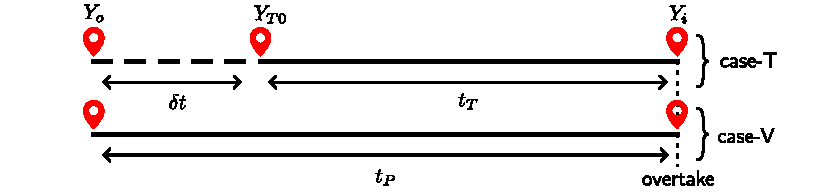
\includegraphics[width=\textwidth]{figures/pep1_analys.pdf}
            \end{figure} \pause
        \end{column}
        \begin{column}{0.3\textwidth}
            Assuming a point mass model.
            \begin{alertblock}{}
                Yes! If $V_{T0} < V_{yo(V)}$, i.e., $\mu < 0.158$. \newline
                So icy conditions at the end of the hairpin?
            \end{alertblock}
        \end{column}
    \end{columns}

\begin{exampleblock}{}
    For the pendulum term to be "\textit{viable}", $V_{T0} < V_{yo(V)}$. In other words, the topt solution?
\end{exampleblock}

\end{frame}